\chapter{Machine Learning and Latent Space Equilibrium}
%
\begin{quote}
"It is widely believed that the real-world data is generated by a few explanatory factors which are distributed, invariant and disentangled" (Bengio et al., 2013).
\end{quote}
%
As previously described in the introductory chapter of this manuscript we have been spectators of a deep advance in the computation technology in this decade that opened for data-science the era of \textbf{big data}. For example there are millions of autonomous software components that continuously crawl the internet network decoding HTML pages from 60 billion of pages collected and indexed in a single database. Each time we capture a picture this file is automatically classified and stored in a cloud space that is claimed to receive 1.2 billion of pictures per day. 

We can define ML as the available set of tools that analyzing such big amount of information are automatically providing a possible uncovered pattern among them to be eventually able to predict a future output of the system and operate any other kind of decision based on data uncertainty. The intimate meaning of \textit{machine learning} in this context is referred to the fact that the human intervention is on the very base of the algorithm structural definition while it is the actual model itself that stitches to the input data.  
%
In science, there are essentially two modelling approaches: \textbf{data driven models}; and \textbf{process based models}.
Although physical modeling is the main primary tool to understand the behaviour of natural processes, and to make inference about the future outcomes, it is becoming an increasingly exploited solution to employ a data driven approach where the process based physical models appear to be not detailed enough to describe complex systems in operational situations. For instance we often look at the sole main physical phenomenon where the output measured quantities are actually corrupted by non linear cascade of underlying effects, or we are even looking at an unknown behavior for witch the model results to be a partial or wrong description for the actual measured representation. 
In some other cases, a hybrid version of combined physical and statistical model could be also explored, as we will see in the next sections. But the actual point is that we start to look at the measures of an experiment, not only from the perspective of the single independent experience but from a more general point of view that takes into account the whole repetition history and a wider operational space.  



\section{Statistical description of DNN}

As already anticipated, in order to gather a wide range of all the possible concurring physical causes that drive the measures, we decided to make use of the latest novel approach of Deep Neural Networks. As a preliminary backward step, this section would provide a slight general description that bases this approach in a statistical oriented fashion. Indeed this is the preferred mathematical representation of the recurrent/repeatable output of a scientific experiment lead by the probability theory as it was generalized by Pierre Laplace (1812). 

The collated set of all measures along the consecutive experimental repetitions is often referred as the model \textit{dataset}, while a single instance of this dataset with a proper selection of the quantities under analysis is commonly called \textit{features} or \textit{covariates}\footnote{The most precise definition seems to be the term covariate used in Analysis of Covariance, a type of General Linear Model in which the independent variables of interest are categorical, but you also need to adjust for the effect of an observed, continuous variable–the covariate}.
%
If we consider our dataset in the generic physical model outputs we can refer as the single input feature of the ML model as a stochastic vector $\bm{x} = [x_1,x_2, ... ,x_N]$ that is characterized by its probability density distribution $p(\bm{x})$. The very general macroscopic description of any machine learning application consists to feed a statistical model with this input feature eventually providing as output the \textit{p.d.f} of another related measure $p(y|\bm{x})$ or a description of $p(\bm{x})$ itself. These two kinds of results are respectively representative of the so called  \textbf{supervised} and \textbf{unsupervised} learning: in the former the the model is confronted with a known relation between variables, while any information is provided to the model for the latter but we are simply looking at the distribution of the variables in their own manifold or in a subspace (as it will described in the next sections).

The unitary element that composes either the standard \textit{Neural Network} structure and the \textit{Deep Neural Network} is the so called \textit{Single Layer Perceptron}; in the following it will be shown that this particular element can be seen as a single instance of a \ac{GLM}, while the operation performed by each of this quantity is a generic regression model applied on its input features.
%
Although GLM is the generalized representation of the ordinary linear regression we shall first introduce the latter as a first example to present the formalism in a simpler manner.
The very basic linear regression model is a linear mapping from N-dimensional input features (or covariates) $\bm{x}$, to a set of targets (or responses) $\bm{y}$, using the inputs, a set of weights (or regression coefficients) $\bm{w}$ and a bias offset $w_0$. The internal product of features and weights gives the equation of the fitter that in the linear form has the shape of a line in the N-dimensional space. The line is centered within the input data while typically the probabilistic model assumes that the residuals can be described with a Gaussian shape of unknown variance $\sigma^2$. The model can be written as a predictor in the form:
\begin{equation}
    \hat{y} = \eta + \epsilon
\end{equation}
where
\begin{equation}
     \eta = \transpose{\bm{w}}\bm{x} \qquad  \epsilon \in \mathcal{N}(0,\sigma^2)
\end{equation}
the first addendum is the \textit{linear predictor} in which a scalar is appended at the end of the the weight vector to fit the bias of the distribution, and the second addendum represents the overall error. To let the model fitting also the bias the parameters and covariates array have been rewritten as follows:
\begin{equation}
    \bm{w} = [\hat{\bm{w}},w_0] \qquad \bm{x} = [\hat{x}, 1]
\end{equation}
At this point the conditional probability of the target given the features can be modeled as a Gaussian distribution:
\begin{equation}
    p(y|\bm{x}) = \mathcal{N}(\eta, \sigma^2)
\end{equation}
this happens because we forced to consider the features with normal distribution and because being an exponential distribution it is also a conjugate prior for the likelihood, as it will described in the following.

\subsection{Generalized Linear Models}
The use of exponential distribution turns to be a very clever solution. Indeed, among all families of distributions, where the definition domain does not vary with the parameter being estimated, this family is the only one with a sufficient statistic whose dimension remains bounded if the sample size increases. This means that we can have a compressed representation of the dataset into a fixed size summary without loss of information.
Exponential families are also important in Bayesian reconstruction where a prior distribution is multiplied by a likelihood function and normalised to produce the posterior. In the case of a likelihood which belongs to an exponential family there always exists a conjugate prior, which is usually also exponentially distributed. 
%
%A conjugate prior for the parameter $\eta$ of an exponential family
The formal definition of a generic exponentially distributed p.d.f. is the following:
%% EXPONENTIAL
\begin{equation}
    p(x|\theta) = \frac{1}{Z(\bm{\theta})}h(x) \exp{[\transpose{\bm{\theta}} \phi(\bm{x})]}
\end{equation}
where $\bm{\theta} \in \Theta \subseteq \mathbb{R}^d$ are defined as the \textbf{natural parameters}, $\phi(\bm{x}) \in \mathbb{R}^d$ is called the vector of \textbf{sufficient statistics}, $h(\bm{x})$ is a scaling factor that is usually a unitary constant, and $Z(\bm{\theta})$ is the \textbf{partition function} that normalizes the distribution:
\begin{equation}
    Z(\bm{\theta}) = 
    \int_{\mathcal{X}^n} h(\bm{x}) \exp{[\transpose{\bm{\theta}} \phi(\bm{x})]} dx
\end{equation}
Being all the arguments within an exponential operator it is also quite common to embed the partition function too, using $ A(\bm{\theta}) = \log\left(Z(\bm{\theta})\right)$ in the following:
\begin{equation}
    p(x|\bm{\theta}) = h(\bm{x}) \exp{[\transpose{\bm{\eta}}\phi(\bm{x}) - A(\bm{\eta}) ]}
\end{equation}
where the function $\eta$ has been further introduced to expand the natural parameters to the representation $\bm{\eta}=\eta(\bm{\theta})$, where $\text{dim}(\bm{\theta}) \leq \text{dim}\left(\eta(\bm{\theta})\right)$.

%% BERNOULLI EXPONENTIAL
\subsubsection*{example: exponential representation of the Bernoulli distribution}
The Bernoulli distribution for $x\in\{0,1\}$ can be written in exponential family form as:
\begin{equation}
\begin{split}
    \text{Ber}(x|\mu) &= \mu^x(1-\mu)^{1-x} \\
%                      &= (1-\mu) \exp{\left[ x \log\left(\frac{\mu}{1-\mu}\right)\right]} \\
                      &= \exp{\left[\transpose{\phi(x)}\bm{\theta} \right]}
\end{split}
\end{equation}
where we set:
\begin{align*}
  & \phi(x) = x \\
  & \theta  = \log\left(\frac{\mu}{1-\mu}\right) \\
  & Z = 1/(1-\mu)
\end{align*}

%% GAUSSIAN EXPONENTIAL
\subsubsection*{example: exponential representation of the Univariate Gaussian distribution}
The univariate Gaussian can be written in exponential family in this form:
\begin{equation}
\begin{split}
        \mathcal{N}(x|\mu,\sigma^2) &= \frac{1}{(2\pi\sigma^2)^\frac{1}{2}} \exp{\left[-\frac{1}{2\sigma^2}(x-\mu)^2\right]} \\
        & \frac{1}{Z(\bm{\theta}}\exp{\left[\transpose{\bm{\theta}}\bm{\phi}(x)\right]}
\end{split}
\end{equation}
once the parameters have been set to:
\begin{align*}
    & \bm{\phi}(x) = \left[ x, x^2 \right] \\
    & \bm{\theta}  = \left[ \frac{\mu}{\sigma^2}, -\frac{1}{2\sigma^2} \right] \\
    & Z(\mu,\sigma^2) = \sqrt{{2\pi\sigma^2}} \exp{\left[ \frac{\mu^2}{2\sigma^2} \right]}
\end{align*}

%%GLM
It has been shown that the linear regression predicts the expected value of a given quantity as a linear combination the dataset. This implies that a constant change in the covariates leads also to a constant change in the response (i.e. a linear-response model). This is appropriate when the response variable has a normal distribution (intuitively, when a response variable can vary essentially indefinitely in either direction with no fixed "zero value", or more generally for any quantity that only varies by a relatively small amount).
However, these assumptions are inappropriate where the response variable is expected to have a different shape. 
% RR
As an example, a prediction model might predict that 10 degree temperature decrease would lead to 1,000 fewer people visiting the beach is unlikely to generalize well over both small beaches (e.g. those where the expected attendance was 50 at a particular temperature) and large beaches (e.g. those where the expected attendance was 10,000 at a low temperature). The problem with this kind of prediction model would imply a temperature drop of 10 degrees would lead to 1,000 fewer people visiting the beach, a beach whose expected attendance was 50 at a higher temperature would now be predicted to have the impossible attendance value of -950. Logically, a more realistic model would instead predict a constant rate of increased beach attendance (e.g. an increase in 10 degrees leads to a doubling in beach attendance, and a drop in 10 degrees leads to a halving in attendance). Such a model is termed an exponential-response model (or log-linear model, since the logarithm of the response is predicted to vary linearly).
%% 
Generalized linear models overcome this limitation extending the ordinary linear models expanding the response variables to any arbitrary distribution (rather than simply the normal), imposing an arbitrary function of the response variable (the link function) to exploit the linearity with the predicted values. 
% RR
For example, the case above of predicted number of beach attendees would typically be modeled with a Poisson distribution and a log link, while the case of predicted probability of beach attendance would typically be modeled with a Bernoulli distribution (or binomial distribution, depending on exactly how the problem is phrased) and a log-odds (or logit) link function.
%%GLM
The three main ingredients of a GLM are:
\begin{itemize}
    \item The \textbf{exponential family} of probability distributions,
    \item the usual \textbf{linear predictor} $\eta = \transpose{\bm{w}}\bm{x}$,
    \item a \textbf{link function} $g$ such that $\expectation{y|\bm{x}} = \mu = g^{-1}(\eta)$.
\end{itemize}

The GLM probability is composed as follows:
\begin{equation}
    p(y_i| \theta, \sigma^2) = 
    \exp{\left[ \frac{y_i\theta - A(\theta}{\sigma^2} + c(y_i,\sigma^2) \right] }
\end{equation}


%
%  _____ ___ _     _       _   _ _____ ____  _____ 
% |  ___|_ _| |   | |     | | | | ____|  _ \| ____|
% | |_   | || |   | |     | |_| |  _| | |_) |  _|  
% |  _|  | || |___| |___  |  _  | |___|  _ <| |___ 
% |_|   |___|_____|_____| |_| |_|_____|_| \_\_____|
%

%% GLM

%% GAUSSIAN MODEL EXAMPLE

%% CLOSED FORM FOR GAUSSIAN MODEL

\subsection{Directed Graphical Models}
In the previous chapter we saw a possible general approach to obtain a regression of a single target variable given its conditional probability with an input process. Suppose now that we are observing a set of multiple correlated variables where the correlation extends from one variable to another in a chain of dependencies. This becomes a stochastic model describing a sequence of possible values for the variables in which the probability of each event depends on the state of the others.
If we constrain the variable correlation to be strictly ordered the probability of a target variable after all the correlation hops can be written as:
\begin{equation}
    p(x_1, x_2, ... x_V | \bm{\theta}) = p(x_1|\bm{\theta})p(x_2|x_1,\bm{\theta})p(x_3|x_2,x_1,\bm{\theta}) ... p(x_V|x_1, ... x_{V-1},\bm{\theta})
\end{equation}
Looking at all the possible $p(x_i|\bm{\theta})$ the conditional links among variable appears as a linked directed graph.
%
This is called “Graphical model” as it combines graph theory and probability theory to provide a general framework to represent variables interaction. Graphical models trace their origins to many different fields and have been applied in wide variety of settings: for example, to develop probabilistic expert systems, and to understand neural networks. Remarkably, the very same formalism and algorithms can be applied to a wide range of problems.
%
However even if the pictorial result is quite intuitive, the joint relation among stochastic variables can easily grow exponentially; for instance if we imagine all distributions having the same finite discrete support composed by $K$ states the representation of all $p(x_i|x_j)$ is $O(K^2)$, the representation of $p(x_i|x_j,x_k)$ is $O(K^3)$ and so forth, so the overall model of V cardinality would become $O(K^V)$. This description of joint discrete possible states, known as the \textbf{conditional probability table}, is sometimes used to describe a fully observed covariates vector in the complete statistical description of the complex systems of variable. Actually this solution, beside requiring a first restriction in the number of possible states that represents each stochastic process, it is also presenting a critical convergence requiring a awful amount of data to reach a meaningful state for such amount of parameters.
One possible solution, in the same discrete approximation, is to make use a more compact conditional distribution function, such as the multinomial logistic i.e. $p(x_i | \bm{x_j})_{i \neq j} = S_k(\bm{W}_i \bm{x_{j}}$). Although this model has been successfully applied in literature for some generative classifiers~\cite{Bengio:1999:MHD:3009657.3009714}, it appears to remain an overkill in conditioning the system.

Another practical end very common solution is to assume a conditional Independence among variables that are k-hops distant from the others, exploiting the \textbf{Markov assumption} of independence among the link graph.
For example, under these conditions, imposing a single hop Independence, the chains of links that create are constituted by first order \textbf{Markov chain} shown in the first diagram of \Figure{\ref{fig:simple_markov_chains_a}}, and described by the following joint distribution:
\begin{equation}
    p(x_1, x_2, ... x_V) = p(x_1) \prod_{j=1}^V p(x_j|x_{j-1})
\end{equation}
equivalently the second order independence can be imposed, generating a graph like in \Figure{\ref{fig:simple_markov_chains_b}} describe by:
\begin{equation}
    p(x_1, x_2, ... x_V) = p(x_1) \prod_{j=1}^V p(x_j|x_{j-1},x_{j-2})
\end{equation}
In the same way higher-order Markov models can be created, however even the second-order Markov assumption may be inadequate if there are long-range correlations throughout the available observations since the number of parameters will again blow up. 





\begin{figure}
    \centering
    \subfigure[]{
    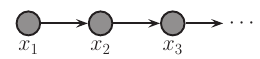
\includegraphics[width=0.3\textwidth]{img/3_ML/DGM_o1_markov.png}
    \label{fig:simple_markov_chains_a} }
    \subfigure[]{
    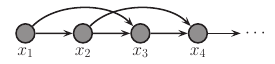
\includegraphics[width=0.3\textwidth]{img/3_ML/DGM_o2_markov.png}
    \label{fig:simple_markov_chains_b} }
    \caption{First order (a) and second order (b) Markov Chain examples, the arrow represents a conditional probability that relates variables each other.}
    \label{fig:simple_markov_chains}
\end{figure}

\begin{figure}
    \centering
    \subfigure[]{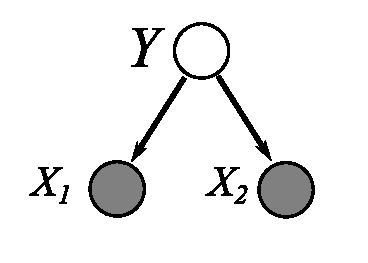
\includegraphics[height=2cm]{img/3_ML/naive_bayes_1.pdf}
    \label{fignaive_bayes}}
    \subfigure[]{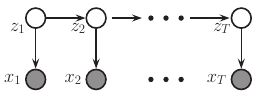
\includegraphics[height=2cm]{img/3_ML/DGM_o1_hmm.png}
    \label{fig:hidden_markov}}
    \caption{Caption}
\end{figure}

A further possible reduction in the number of joint relations between observed variables can be also given by the formalism itself,  by the assumption that some covariates are correlated because they all arise from a hidden common “cause”. Those common causes are variables themselves that can't be directly measured.  Model with hidden variables are also known as latent variable models or LVMs. 

The actual very powerful alternative approach is to assume that there is an underlying hidden process, that can be modeled by a first-order Markov chain, but for which available measures is a noisy observation of this process. The result is known as \acl{HMM}, shown in \Figure{\ref{fig:hidden_markov}}. 










%  _____ _____ ____  _   _      _                      _    
% |  ___|  ___|  _ \| \ | | ___| |___      _____  _ __| | __
% | |_  | |_  | | | |  \| |/ _ \ __\ \ /\ / / _ \| '__| |/ /
% |  _| |  _| | |_| | |\  |  __/ |_ \ V  V / (_) | |  |   < 
% |_|   |_|   |____/|_| \_|\___|\__| \_/\_/ \___/|_|  |_|\_\

\subsection{Feed forward dense network}
%

Feedforward neural networks such as multilayer perceptrons are popular tools
for nonlinear regression and classification problems. From a Bayesian per-
spective, a choice of a neural network model can be viewed as defining a prior
probability distribution over nonlinear functions, and the neural network’s
learning process can be interpreted in terms of the posterior probability dis-
tribution over the unknown function. (Some learning algorithms search for the
function with maximum posterior probability and other Monte Carlo methods
draw samples from this posterior probability.)
In the limit of large but otherwise standard networks, Neal (1996) has
shown that the prior distribution over nonlinear functions implied by the
Bayesian neural network falls in a class of probability distributions known
as Gaussian processes. The hyperparameters of the neural network model
determine the characteristic lengthscales of the Gaussian process. Neal’s ob-
servation motivates the idea of discarding parameterized networks and working
directly with Gaussian processes. Computations in which the parameters of
the network are optimized are then replaced by simple matrix operations using
the covariance matrix of the Gaussian process.

A feed forward NN, aka \ac{MLP} is again using the linear regression, actually it can be seen as a chain of logistic regression models that are stacked one on top of each other, where the final layer being a \ac{GLM}, either a logistic or a linear regression depending weather we are looking for a general classification output (i.e. a probability function output for each of the classes in the classifier domain) or a regression output. 
For instance, looking at the simple two layers example, and considering a regression output problem, the model would be written like:
\begin{equation}
    p(y|\bm{x},\bm{\theta}) = \mathcal{N}\left(y|\transpose{\bm{w}}\bm{z(\bm{x}}), \sigma^2 \right)
    \label{eq:mlp_a}
\end{equation}
where the basis function expansion here is a non-linear response of further linear combination of the inputs:
\begin{equation}
    \bm{z}(\bm{x}) = \left[ g(\transpose{\bm{v}_1}\bm{x}), g(\transpose{\bm{v}_2}\bm{x}), ..., g(\transpose{\bm{v}_H}\bm{x})
    \right]
    \label{eq:mlp_b}
\end{equation}
the transformation $z(\bm{x})$ represents here the non-linear transformation on regression in which the deterministic function $g(\bm{x},\bm{v})$, also called the \textbf{activation function}, is the kernel of the basis function expansion. In this way we could think of the \acl{MLP} as a kernel machine where the kernel functions have been opportunely shaped to match the input data. This parametrization on the kernel function makes the \acl{MLP} an \ac{ABM}:
\begin{equation}
    f(\bm{x}) = \transpose{\bm{w}}\bm{\phi}(\{1,\bm{x}\}, \bm{V})
\end{equation}
The generic basis function $\phi(\bm{x},\bm{V})$ must be trained on the dataset to make it "adapt" at the input statistics; while
the entire parameter set that embrace the kernel is now: $\bm{\theta} = (\bm{w}, \bm{v})$ with $\bm{w} = [w_0, w_1, ..., w_M]$ and $\bm{v}_m = [v_{m1}, v_{m2}, ..., v_{mH}]$. The first set of parameters are the linear combination coefficients of the \ac{GLM}, and the second are the parametrization of the kernel. The unit appended to the input feature has been used to add the bias coefficient $w_0$.

\begin{figure}
    \centering
    \subfigure[]{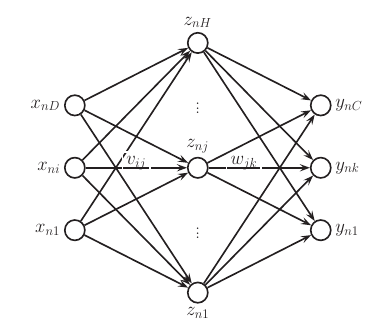
\includegraphics[height=4cm]{img/3_ML/MLP.png} \label{fig:mlp_a}}
    \subfigure[]{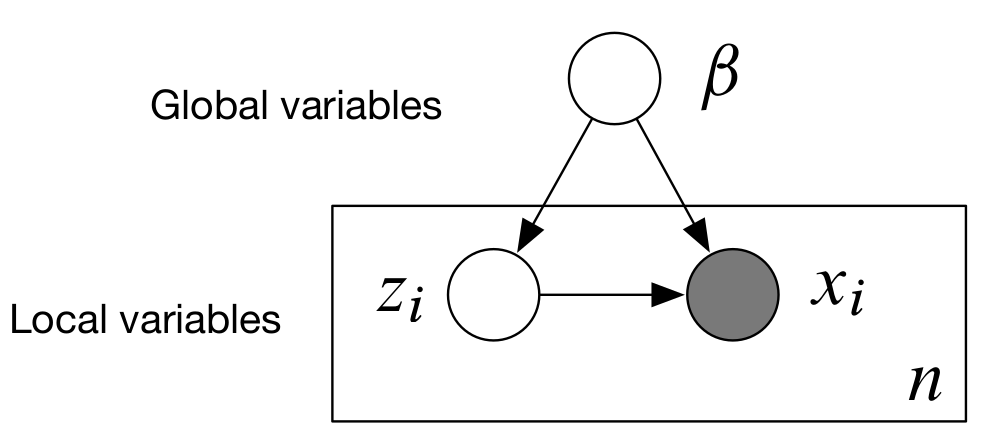
\includegraphics[height=4cm]{img/3_ML/FDN_plate_model.png}}
    \caption{One hidden layer Feed Forward Neural Network (or equivalently the minimal Multi Layer Perceptron, seen as an Adaptive Basis Function Model (a), and the equivalent model in plate notation (b). }
    \label{fig:mlp}
\end{figure}

The final \acl{GLM} applied can be constructed as usual in many different shapes, depending on the target type of inference we are interested in. If we look for a binary classification it appears as a logistic regression, i.e. the fit on the Bernoulli distribution of the sigmoid outputs:
\begin{equation}
    p(y|\bm{x}, \bm{\theta}) = \text{Ber}\left( y|\text{sigm}(\transpose{\bm{w}}\bm{z}(\bm{x}) \right)
\end{equation}
If we are looking for categorical classifier the correct GLM has to be distributed as:
\begin{equation}
    p(y|\bm{x}, \bm{\theta}) = \text{Cat}\left( y|\mathcal{S}(\transpose{\bm{w}}\bm{z}(\bm{x})) \right)
\end{equation}
where the \textit{Cat} distribution is the Multinulli and $\mathcal{S}$ stands for the support function of the input.
Finally as stated in the first example if we are fitting a generic output function it will appear for example as a Gaussian regression model:
\begin{equation}
    p(\bm{y}|\bm{x}, \bm{\theta}) = \mathcal{N}\left( \bm{y}|\bm{W} \phi \right)
\end{equation}
where in this last version of the formula the probability has been shaped with the weights matrix $\bm{W}$ taking into account the possible MIMO configuration of the perceprton as shown in \Figure{\ref{fig:mlp_a}}.
It is finally a key factor for the activation function $g(\bm{x},\bm{v})$ to be a non-linear operator because the overall network would collapse into a large linear regression otherwise. Usually the activation is the logistic function $g(u) = \text{sigm}(u)$ or the recently much common flavors of the \textbf{rectified linear units} (ReLU) that provide a non linear activation with a minimal computational effort.
%
% SHOW A FIGURE OF THE POSSIBLE ACTIVATION FUNCTIONS
% 
All this kind of complication that have been added to the simple GLM are eventually building an optimization problem, finding the best functional fit for a set of input-output examples. So what we are doing at a very general level is tuning the weights to chase for an optimal configuration; but two complementary motivations determine what \textit{optimal} means in this context. On the one side we want the network to represent the target as exactly as possible. But on the other hand the network must be also \textbf{capable of generalize}, that is, when unknown inputs must be compared to the known producing an output that is a kind of interpolation of learned values. However, good generalization and minimal reproduction error of the learned input-output pairs can become contradictory objectives as already briefly discussed about the fitting of the network to the data (i.e. over-fitting and under-fitting training).
A more detailed discussion is postponed to \cref{section:training_regularization}
%

%% tell something about the cost function

%  _                _                          
% | |__   __ _  ___| | ___ __  _ __ ___  _ __  
% | '_ \ / _` |/ __| |/ / '_ \| '__/ _ \| '_ \ 
% | |_) | (_| | (__|   <| |_) | | | (_) | |_) |
% |_.__/ \__,_|\___|_|\_\ .__/|_|  \___/| .__/ 
%                       |_|             |_|    

\subsection{Optimization of parameters and the backpropagation algorithm}

In the previous section the the basic structure of a \acl{MLP} has been presented as a particular adaptive kernel version of the \acl{GLM}, however unlike this one the negative log-likelihood of a \acl{MLP} is a non-convex function of the parameters. It is nevertheless always possible to obtain a local maximum of the posterior probability locating the minimum of a cost function in a gradient-based optimization procedure. 
To proceed toward a descent path on a gradient vector of the negative log-likelihood is needed. This can be obtained in several ways, but it is a very common approach for NN to exploit the fact that the internal hidden units of a \acl{MLP} form a chain rule of calculus. The resulting algorithm is known as the \textbf{backpropagation} an it will be presented n the following as it has been the method used in all the results presented in this document. The backpropagation is a method to compute the variation of the cost function with respect to a variation on the single neuron unit, so one could think that all hidden units as statistically described by internal states variables providing a stochastic version of the descent algorithm~\cite{rezende2014stochastic}; however in this brief description we will consider the hidden units as a part of the adaptive kernel of the \acl{MLP} as described, so that the optimum has only to be found among the gradients of all units function (i.e. the linear combination of coefficients and the activation function). 

To obtain a simple notation we will assume in the next the model as it was presented in \Figure{\ref{fig:mlp_a}}: with just a single hidden layer. This will be indeed helpful to separate the \textit{pre-synaptic} and \textit{post-synaptic} entities of neurons, that are, values of the signal passing through, before and after we apply the non-linearity of the activation function. Let $\bm{x}_n$ be the n\'th input, $\bm{a}_n = \bm{V}\bm{x}_n$ the \textit{pre-synaptic} hidden layer, and $\bm{z}_n = g(\bm{a}_n)$ be the \textit{post-synaptic} hidden layer, where $g$ is some transfer function. 
For the activation function, as already discussed, several non linear function is commonly used: the classical literature presents $g(a) = sigm(a)$, or equivalently $g(a) = tanh(a)$, but we also stated that a common modern solution is to exploit the ReLU or Leaky-ReLU functions. 
We will now consider the model as presented in \Equation{\ref{eq:mlp_a}}; the pre and post synaptic outputs can be divided as: $\bm{b}_n = \bm{W}\bm{z}_n$ pre-synaptic output, and $\hat{\bm{y}}_n = h(\bm{b}_n)$ the post-synaptic output. In the second term we also represented the non linear effect of the \acl{GLM} canonical link function as $h$.
In the regression case of \acl{GLM} the negative log-likelihood appears as the \textbf{mean squared error} of the signal that passed through the network with the ground truth:
\begin{equation}
    J(\bm{\theta}) = -\sum_n\sum_k \left(\hat{y}_{nk}(\bm{\theta}) - y_{nk}\right)^2
\end{equation}
Otherwise in the classification case the negative log-likelihood assumes the typical form of the \textbf{cross entropy} between the reconstruction output and the actual real class of each sample:
\begin{equation}
    J(\bm{\theta}) = -\sum_n\sum_k y_{nk} \log \hat{y}_{nk}(\bm{\theta})
\end{equation}
%
Let us start by considering the output layer weights from the \acl{GLM}:
\begin{equation}
    \nabla_{\bm{w}_k} J_n = \pdv{J_n}{b_{nk}} b_{nk} = \pdv{J_n}{b_{nk}} \bm{z}_n
\end{equation}
where $b_{nk} = \transpose{\bm{w}_k}\bm{z}_n$ and, considering all the chained relations, it can be shown ( see GLM ML ) that the the derivative can be set to:
\begin{equation}
    \pdv{J_n}{b_{nk}} = ( \hat{y}_{nk} - y_{nk} ) \triangleq \delta_{nk}^w
\end{equation}
and the overall gradient with respect to the output signal is:
\begin{equation}
    \nabla_{\bm{w}_k} J_n = \delta_{nk}^w \bm{z}_n
\end{equation}
A similar procedure can be also applied to the input layer:
\begin{equation}
    \pdv{J_n}{a_{nj}} = \sum_{k=1}^K \pdv{J_n}{b_{nk}}\pdv{b_{nk}}{a_{nj}} 
    \triangleq \sum_{k=1}^K \delta_{nk}^w \pdv{b_{nk}}{a_{nj}}
\end{equation}
Now we introduce the actication function at the input of the link function, so from the defined $b_{nk}$ as:
\begin{equation}
    b_{nk} = \sum_j w_{kj} g( a_{nj} )
\end{equation}
the derivative becomes:
\begin{equation}
    \pdv{b_{nk}}{a_{jk}} = w_{kj} g^\prime(a_{nj})
\end{equation}
The derivative of the activation function varies for the specific case; for example:
\begin{align*}
    & \pdv{}{a} \tanh(a) = 1-\tanh^2(a) \\
    & \pdv{}{a} \text{sigm}(a) = \text{sigm}(a)(1-\text{sigm}(a))
\end{align*}
Hence:
\begin{equation}
    \delta_{nj}^v = \sum_{k=1}^K \delta_{nk}^w w_{kj} g^{\prime}(a_{nj})
    \label{eq:backprop_error}
\end{equation}
Putting it all together, we can compute all the gradients as follows: we first perform a forward pass to compute $a_n$ , $z_n$ , $b_n$ and $\hat{y}_n$. We then compute the error for the output layer, $\delta_n^{(2)} = \hat{y}_n - y_n$, which we pass backwards through $\bm{W}$ using \eqref{eq:backprop_error} to compute the error for the hidden layer $\delta_n^{(1)}$. We then compute the overall gradient as follows:
\begin{equation}
    \nabla_{\bm{\theta}} J(\bm{\theta}) = \sum_n \left[ \bm{\delta}_n^v \bm{x}_n, \bm{\delta}_n^w \bm{z}_n \right]
\end{equation}

It is also quite straightforward to see that the parameters are not uniquely identifiable. For example, we can change the sign of the weights going into one of the hidden units, while changing the sign of all the weights out of it; these composed effect cancels. Similarly, we can change the identity of the hidden units without affecting the likelihood. 
In addition, there may be local minima due to the general non-convexity of the log-likelihood. This can be a more serious problem, although with enough data, these local optima are often quite “shallow”, and simple stochastic optimization methods can reach the optimal value of the parameters.



%                       _            _          _   _             
%  _ __ ___  __ _ _   _| | __ _ _ __(_)______ _| |_(_) ___  _ __  
% | '__/ _ \/ _` | | | | |/ _` | '__| |_  / _` | __| |/ _ \| '_ \ 
% | | |  __/ (_| | |_| | | (_| | |  | |/ / (_| | |_| | (_) | | | |
% |_|  \___|\__, |\__,_|_|\__,_|_|  |_/___\__,_|\__|_|\___/|_| |_|
%           |___/                                                 

\subsection{Regularization}
\label{section:training_regularization}
Both in the introductory chapter and the previous section the concept of generalization and fitting the network has been introduced, a more detailed description of the phenomenon and the approach used to provide a solution are described in the following.
The general operation of making the network "generalizing" well over unknown inputs is generally referred as the \textbf{regularization}. It is actually a complex argument that spans across different aspects on network engineering; such as: the dataset organization, the activation selection, the network topology shaping, the internal layers operations, etc. 

We will also distinguish two main kinds of regularization in the following: the \textbf{training regularization} as all the action that play during training, for example by reordering dataset, changing learning rate, or adding operands to the loss function; and the \textbf{network regularization} as all possible permanent modifications to the network that continue to hold also after the training is concluded. Examples of the latter case are for example deep modification of the network behavior, like the introduction of convolutions layers or further action performed after the activation function, such as the Batch normalization. 
Some regularization techniques, as the ones just exposed, have been effectively used during the tests presented in the manuscript so we will be briefly present them in the next sections.

\subsubsection{Adaptive moment optimization}
In the previous section the general approach known as the backpropagation algorithm that provides the gradient to search for maximum likelihood, or equivalently the minimum loss function, has been explained. 
The algorithm outputs a value for the parameters update in the iterative steps of the gradient descent; this gradient is then applied by a learning factor that act as a learning regularization. This parameter is usually fine tuned to provide a good global minimum of the loss function.
Usually the stochastic gradient descent varies the learning rate during the training epochs, for example it undergoes a reduction on the plateau of the learning curve expressing a sort of annealing of the parameters updates; a typical solution is to apply a simple callback function that uses the epoch number and the loss values to iteratively update the learning factor.
Although this simple principle appears quite easy, and it is already provided by some frameworks such as \textit{keras}, it presents some difficulties such as the fact that it can't be effectively applied on the actual plateau but only at fixed times (i.e. end of epoch) during training, and more important it does not automatically account the possible noise associated to the instant loss value of a poorly regularized training.
A different method that recently gained lot of attention was presented by Diederik Kingma (2015) called \textbf{Adam} ( a contraction for "\textit{adaptive moment estimation}")~\cite{kingma2014adam}. This specific formulation can be used instead of the classical stochastic gradient descent procedure to update network weights based on the training dataset; it computes individual adaptive learning rates for parameters exploiting the estimates of first and second order moments of the gradients. 
We choose to apply this method during the tests performed, thanks to the computational efficiency, the little memory required for the run, and because it appears to be very flexible where the dataset use to present noisy gradients.
Specifically, the algorithm calculates an exponential moving average of both the gradient value and its squared, and further global parameters $\beta_1$ and $\beta_2$ control the decay rates of these moving averages. 
The initial value of the moving averages and the control parameters are usually close to 1.0 resulting in a bias of moment estimates towards zero. This bias is overcome by first calculating the biased estimates before then calculating bias-corrected estimates.
If we set the computed gradients of the backpropagation algorithm as:
\begin{equation}
    g_t = \nabla_{\bm{\theta}} f_t(\bm{\theta_{t-1}})
\end{equation}
it computes the estimates of the moments as:
\begin{align}
    & m_t = \frac{\beta_1 m_{t-1} + (1 - \beta_1) g_t  }{1-\beta_1} \\
    & v_t = \frac{\beta_2 v_{t-1} + (1 - \beta_2) g_t^2}{1-\beta_2}
\end{align}
the update of parameters is applied as:
\begin{equation}
    \bm{\theta}_t = \bm{\theta}_{t-1} - \alpha \left( \frac{m_t}{v_t^\frac{1}{2} + \epsilon} \right)
\end{equation}
So the moving averages themselves are estimates of the first moment ( $m_t$ ) and the second raw moment (uncentered variance $v_t$) of the gradient.  However, this average is initialized as zero vectors, leading to a bias on moment estimates, especially during the initial steps, and in particular the effect is higher the smaller the decay rates. This initialization bias is counteracted by the denominator of the estimates as it can be shown that being the first moment:
\begin{equation}
    m_t = (1 - \beta_1) \sum_{i=1}^t \beta_1^{t-1} \cdot g_i
\end{equation}
The average is:
\begin{align*}
    \expectation{m_t} &= \expectation{g_t} \cdot (1-\beta_1) \sum_{i=1}^t \beta_1^{t-1} + \zeta \\
                      &= \expectation{g_t} \cdot (1-\beta_1) + \zeta
\end{align*}
and the derivation for the second moment estimate is completely analogous.
Here the $\zeta$ is a coefficient that does not depend on the gradient moments and $\zeta = 0$ if it is stationary; otherwise it can be kept small since the exponential decay rate $\beta$ can (and should) be chosen such that the exponential moving average
assigns small weights to gradients too far in the past. Therefore the algorithm divides as stated by this term to correct the initialization bias.


\subsubsection{Convlutional layers}

The previous sections explained how the \ac{ABM} hidden units are able to learn non-linear combinations of the original inputs; this is generally referred as the process of \textbf{feature extraction}. In this context the extraction means that the hidden units provide the tempered features for the input of the final \ac{GLM}. 
%
And thanks to the properties of the fully connected network, and in particular to the universal approximation theorem, this approach proves to be particularly effective, specially for problems where the original input covariates are not very individually informative. 
Although the real power NNs is acting out the non-linear relations on input signals, for a task where there is a strong sequential correlation among covariates, extracting “higher order” features with fully connected neurons is less important.
%
The convolutional layers - the basis of famous \ac{CNN} models like AlexNet~\cite{Krizhevsky:2012:ICD:2999134.2999257}, GoogleNet/inception~\cite{7298594} -, are yet another example of this concept, thus it should not be surprising fact that it actually behave like a means of network regularization.
%
As what has been just presented about Adam optimizer, typical ways of regularization include adding some form of magnitude measurement of weights to the loss function. However this is not the sole way to make the network output more general; \acl{CNN} networks take a different approach for regularization: they take advantage of the hierarchical pattern within the data to represent complex patterns using smaller and simpler ones. 
In more detail convolutional networks are simply neural networks that use convolution in place of general matrix multiplication in at least one of their hidden layers.
For a 2D-image for instance the \textbf{convolutional layers} have hidden units with \textbf{local receptive field} where the learning parameters (i.e. the $\bm{V}$ matrix of convolution layers) are tied together in the convolution kernel and thus share across the image. Intuitively, the effect of such spatial relation is that any useful features that are “discovered” in a portion
of the image can be re-used everywhere else without having to be learned independently. The resulting networks then exhibit a translation invariance - they are also referred as \textbf{space invariant artificial neural networks} (SIANN) - meaning they can recognize patterns no matter where they are occurring within the input.
The same holds for 1D-signals too, as a similar spatial relation can be made explicit as well.

So convolutional layers are a form of regularization in the sense that, while for a \ac{MLP} the fully connected network ( where each neuron in one layer is connected to all neurons in the next) makes it prone to overfit data, in \ac{CNN} the effect of sharing parameters along the features could be eventually compress the network complexity. Or equivalently a small network with convolutional layers, thanks to external assumptions on the nature of the data, can act like a bigger one with a more complex behavior.
%
In addition it will be shown - and is the actual main target of the present study - how the very deep joint relations among features can be easily managed by \ac{DNN} without handling the complex models that drive the experimental outcomes; but that we can also make the frequentists approach (i.e. stochastic modeling) closer to the physical and theoretical aspects of experiments with regularization.

\subsubsection{Dropouts}
Being the nature of NN training a deep stochastic process, it is also prone to find different solution of the same problem, depending for example on the initial conditions. This eventually leads to possible local minima. 
Dropout is another cleaver network regularization method that makes the training process behave like it were contemporaneously training a large set of neural networks with different architectures in parallel.
By dropping a unit out, we mean temporarily removing it from the network, along with all its incoming and outgoing connections.
So, during training, some number of layer outputs are randomly ignored or as the name says they are “dropped out”. This has the effect that in each attempt the actual layer that plays in optimization looks-like a layer with a different number of nodes and connectivity with respect to the previous one. In last effect, each update to a layer during training is performed with a different “view” of the configuration as the overall network were a different one.

\begin{lstlisting}[language=Python, caption=Dropout layer code example (from Tensorflow 2.0)]
@tf_export("nn.dropout", v1=[])
def dropout_v2(x, rate, noise_shape=None, seed=None, name=None):
    [...]
    random_tensor = random_ops.random_uniform( noise_shape, 
                                               seed=seed, 
                                               dtype=x.dtype )
    keep_prob = 1 - rate
    scale = 1 / keep_prob
    keep_mask = random_tensor >= rate
    return = x * scale * math_ops.cast(keep_mask, x.dtype)
\end{lstlisting}

\subsubsection{Batch normalization}
A further method to increase the stability (read generalization) of a neural network is the \textit{batch normalization}~\cite{ioffe2015batch} layer. It normalizes the output of the previous activation by subtracting the mean and dividing by the standard deviation computed on the mini-batch.
However, after this shift and scale of the activation output - that are operated by some randomly initialized parameters - the weights in the next layer may be no longer optimal. The optimization process so tends to destroy this normalization if it move the output away from the loss function minimum.
As stated, the batch normalization adds two further trainable parameters where applied: the normalized output is multiplied by a “standard deviation” parameter ( $\gamma$ ) and add a “mean” parameter ( $\beta$ ). In other words, batch normalization lets stochastic gradient do the de-normalization by changing only these two weights for each activation, instead of losing the stability of the network by changing all the weights.
Here we compute the moments of the hidden layers outputs over the mini-batch as:
\begin{align*}
    & {\mu_l}_{\text{BN}} = \expectation{\bm\phi_l(\bm{x})} \\
    & {\sigma^2_l}_{\text{BN}} = \expectation{ (\bm\phi_l(\bm{x}) - {\mu_l}_{\text{BN}})^2 }
\end{align*}
where we wrote with $\phi_l(x_i)$ the i-th activation output of the l-th layer where BN is applied.
Then we apply the normalization:
\begin{equation}
    \hat{x_i} = \frac{x_i - {\mu_l}_{\text{BN}}}{ {\sigma_l}_{\text{BN}} + \epsilon }
\end{equation}
Finally the scale and shift operation is:
\begin{equation}
    y_i = \gamma \hat x_i + \beta
\end{equation}
One effect of the Batch Normalization is to generally increase the training speed as a higher learning rate can be used; this happens because batch normalization constrain activation functions output to a limited support. 

It also reduces over-fitting because, similarly to the Dropout, it adds a noise to each hidden neuron activation. Therefore, if we use batch normalization, we will use less or even any dropout, which is a good thing because we are not going to lose a lot of information. However the two effects are not interchangeable.
%
It is also quite straightforward to see that this kind of regularization layer, as well as the convolutional layer, is a \textbf{network regularizer} thus it must be always kept in the model, even after the end of the training. This represent in a way a limitation of the expression capability because it must be implemented in every running software or hardware support chosen for the final deployment of the network. This could seem a slight drawback because the overall networks grows in parameters, however, aside of the benefit of the regularization, the layer bias coefficient of the linear combination can (an should) be removed because the bias effect is wiped out by the output mean shift.

\subsubsection{Activity regularization}
Activity regularization is instead a \textbf{training regularization} that provides a way to encourage a neural network to learn sparse features or internal representations of raw observations.
It is quite common to push sparsity of representation in autoencoders as we will see in few paragraphs, although the approach can be used also generally both in reducing over-fitting and improving network generalization.

The activity regularization acts on the parameters, i.e. the amplitude of the learned weights, it works on the assumption that smaller weights tends to generate simpler models and thus they helps to avoid over-fitting. So we wants to penalize weights that are actually very close to zero, meaning that we are looking at covariates or internally extracted features that seem not really related to the targets.

We will present here two kinds of such activity regularizers named L1-norm (Lasso regularizer) and L2-norm (Ridge regularizer).
In Lasso we shrink the parameters toward zero; indeed when input features have smaller weights this leads to a sparse L1-norm. Here with sparsity we refer to the weights matrix of the fully connected layers, so in very sparse solutions the majority of the input features have zero weights and very few of them are instead active in the determination of the output.
So in this sense the Lasso regularization performs a feature selection, assigning insignificant input features with zero weight and useful features with a non zero weight:
\begin{equation}
    L_1(x,y) \triangleq \lambda_1 \sum_{i=1}^{H_l} \left| v_i \right|
\end{equation}
In L2 regularization, regularization term is the sum of square of all feature weights:
\begin{equation}
    L_2(x,y) \triangleq \lambda_2 \sum_{i=1}^{H_l} v_i^2
\end{equation}
At the end the overall Loss is composed by the target loss, \textit{mse} for instance, and the sum of all layer losses:
\begin{equation}
    L(x,y) = \sum_{i=1}^N (y_i - \transpose{\bm{w}}\bm{z_i}(\bm{x}))^2 + \lambda_1 \sum_{j=1}^{L1} L_1(x_i,y_i)_j + \lambda_2 \sum_{k=1}^{L2} L_2(x_i,y_i)_k
\end{equation}

These activity regularizers are only affecting the loss and thus they only pertain on training, so they are training regularizers and shall not be deployed in a trained network.
% \begin{lstlisting}[language=Python, caption=activity L1L2 regularizer in keras (tf 2.0)]
% @keras_export('keras.regularizers.L1L2')
% class L1L2(Regularizer):
%   def __call__(self, x):
%     if not self.l1 and not self.l2:
%       return K.constant(0.)
%     regularization = 0.
%     if self.l1:
%       regularization += self.l1 * math_ops.reduce_sum(math_ops.abs(x))
%     if self.l2:
%       regularization += self.l2 * math_ops.reduce_sum(math_ops.square(x))
%     return regularization
% \end{lstlisting}



%  _   _ _   _ ____  _   _ ____  _____ ______     _____ ____  _____ ____  
% | | | | \ | / ___|| | | |  _ \| ____|  _ \ \   / /_ _/ ___|| ____|  _ \ 
% | | | |  \| \___ \| | | | |_) |  _| | |_) \ \ / / | |\___ \|  _| | | | |
% | |_| | |\  |___) | |_| |  __/| |___|  _ < \ V /  | | ___) | |___| |_| |
%  \___/|_| \_|____/ \___/|_|   |_____|_| \_\ \_/  |___|____/|_____|____/ 

\section{Unsupervised learning: Generative modeling}
%
% RR
“Generative modeling” is a broad area of machine learning which deals with models of distributions $p(\bm{x})$, defined over datapoints X in some potentially high-dimensional space X. For instance, images are a popular kind of data for which we might create generative models. Each “datapoint” (image) has thousands or millions of dimensions (pixels), and the generative model’s job is to somehow capture the dependencies between pixels, e.g., that nearby
pixels have similar color, and are organized into objects. Exactly what it means to “capture” these dependencies depends on exactly what we want to do with the model. One straightforward kind of generative model simply allows us to compute P(X) numerically. In the case of images, X values  which look like real images should get high probability, whereas images that look like random noise should get low probability. However, models like this are not necessarily useful: knowing that one image is unlikely does not help us synthesize one that is likely. Instead, one often cares about producing more examples that are like those already in a database, but not exactly the same. We could start with a database of raw images and synthesize new, unseen images. We might take in a database of 3D models of something like plants and produce more of them to fill a forest in a video game. We could take handwritten text and try to produce more handwritten text. Tools like this might actually be useful for graphic designers. We can formalize this setup by saying that we get examples X distributed according to some unknown distribution Pgt(X), and our goal is to learn a model P which we can sample from, such that P is as similar as possible to Pgt.




\subsubsection{Mixture models}



\subsubsection{linear factor analysis}

One problem with mixture models is that they only use a single latent variable to generate the
observations. In particular, each observation can only come from one of K prototypes. One can
think of a mixture model as using K hidden binary variables, representing a one-hot encoding
of the cluster identity. But because these variables are mutually exclusive, the model is still
limited in its representational power.
An alternative is to use a vector of real-valued latent variables, $z_i \in R_L$ . The simplest prior
to use is a Gaussian (we will consider other choices later):

% p(zi ) = N (zi |μ0 , Σ0 )

If the observations are also continuous, so $x_i \in R_D$ , we may use a Gaussian for the likelihood.
Just as in linear regression, we will assume the mean is a linear function of the (hidden) inputs,
thus yielding




% RR  VAE
Training this type of model has been a long-standing problem in the machine learning community, and classically, most approaches have had one of three serious drawbacks. First, they might require strong assumptions about the structure in the data. Second, they might make severe approximations, leading to sub optimal models. Or third, they might rely on computationally expensive inference procedures like Markov Chain Monte Carlo. More recently, some works have made tremendous progress in training neural networks as powerful function approximators through backpropagation \cite{NIPS2012_4824}. These advances have given rise to promising frameworks which can use backpropagation-based function approximators to build generative models. One of the most popular such frameworks is the Variational Autoencoder \cite{}, the subject of this tutorial. The assumptions of this model are weak, and training is fast via backpropagation. VAEs do make an approximation, but the error introduced by this approximation is arguably small given high-capacity models. These characteristics have contributed to a quick rise in their popularity

% RR
An autoencoder is a neural network that is trained to attempt to copy its input to its output. Internally, it has a hidden layer $h$ that describes a code used to represent the input. The network may be viewed as consisting of two parts: an encoder function $h=f(x)$ and a decoder that produces a reconstruction $r=g(h)$. If an autoencoder succeeds in simply learning to set $g(f(x))=x$ everywhere, then it is not especially useful. Instead, autoencoders are designed to be unable to learn to copy perfectly. Usually they are restricted in ways that allow them to copy only approximately, and to copy only input that resembles the training data. Because the model is forced to prioritize which aspects of the input should be copied, it often learns useful properties of the data.
%  _____ ___ _     _       _   _ _____ ____  _____ 
% |  ___|_ _| |   | |     | | | | ____|  _ \| ____|
% | |_   | || |   | |     | |_| |  _| | |_) |  _|  
% |  _|  | || |___| |___  |  _  | |___|  _ <| |___ 
% |_|   |___|_____|_____| |_| |_|_____|_| \_\_____|
%

%% ALL DIMENSIONALITY REDUCTION

% RR
Modern autoencoders have generalized the idea of an encoder and a decoder beyond deterministic functions to stochastic mappings $p_{encoder}(h | x)$ and $p_{decoder}(x | h)$.

%% TODO: TALK ABOUT GAN TOO

\subsection{Variational autoencoders and ELBO minimization}

% RR
In just three years, Variational Autoencoders (VAEs) have emerged as one of the most popular approaches to unsupervised learning of complicated distributions. VAEs are appealing because they are built on top of standard function approximators (neural networks), and can be trained with stochastic gradient descent.

% RR
Copying the input to the output may sound useless, but we are typically not interested in the output of the decoder. Instead, we hope that training the autoencoder to perform the input copying task will result in h taking on useful properties. One way to obtain useful features from the autoencoder is to constrain h to have a smaller dimension than x. An autoencoder whose code dimension is less than the input dimension is called \textbf{undercomplete}. Learning an undercomplete representation forces the autoencoder to capture the most salient features of the training data.







%  _____ ___ _     _       _   _ _____ ____  _____ 
% |  ___|_ _| |   | |     | | | | ____|  _ \| ____|
% | |_   | || |   | |     | |_| |  _| | |_) |  _|  
% |  _|  | || |___| |___  |  _  | |___|  _ <| |___ 
% |_|   |___|_____|_____| |_| |_|_____|_| \_\_____|
%


\section{Latent space topology in a simulated world}

\subsection{STEP1}

\begin{figure}
    \centering
    \subfigure{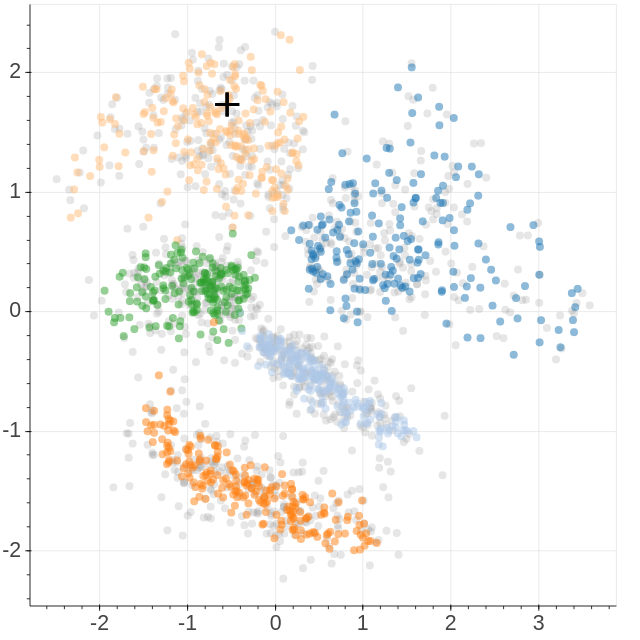
\includegraphics[height=4.5cm]{img/STEP1/ls1.png} \label{step1_1}}
    \subfigure{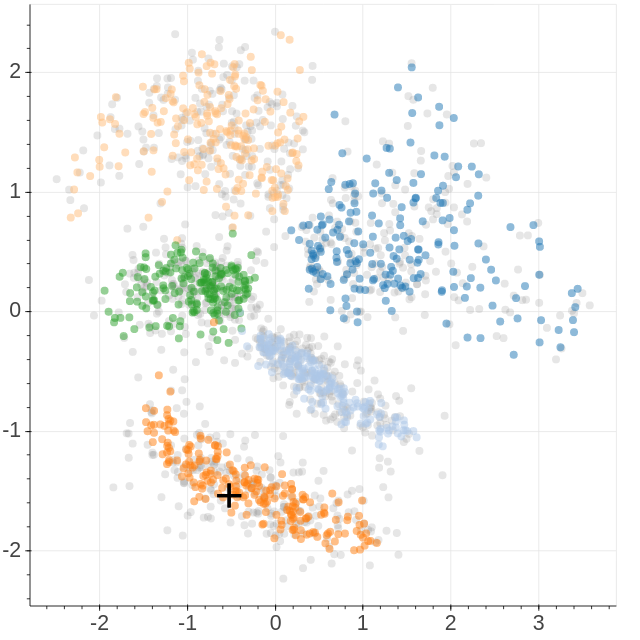
\includegraphics[height=4.5cm]{img/STEP1/ls2.png} \label{step1_2}}
    \subfigure{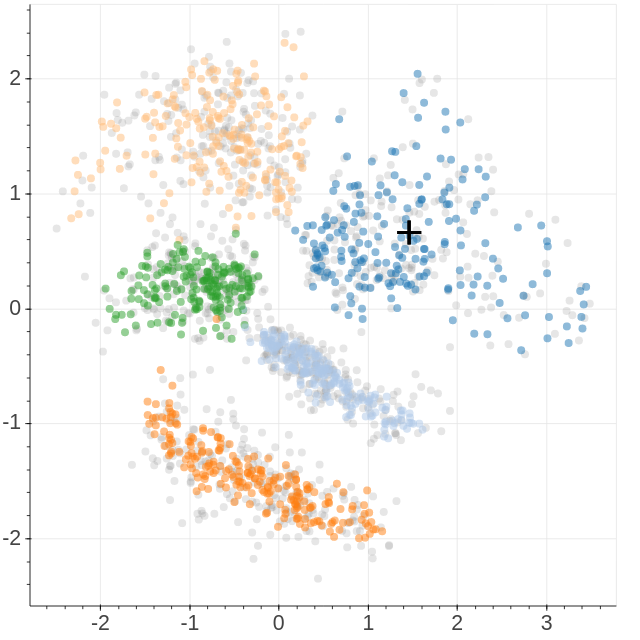
\includegraphics[height=4.5cm]{img/STEP1/ls3.png} \label{step1_3}}
    \subfigure{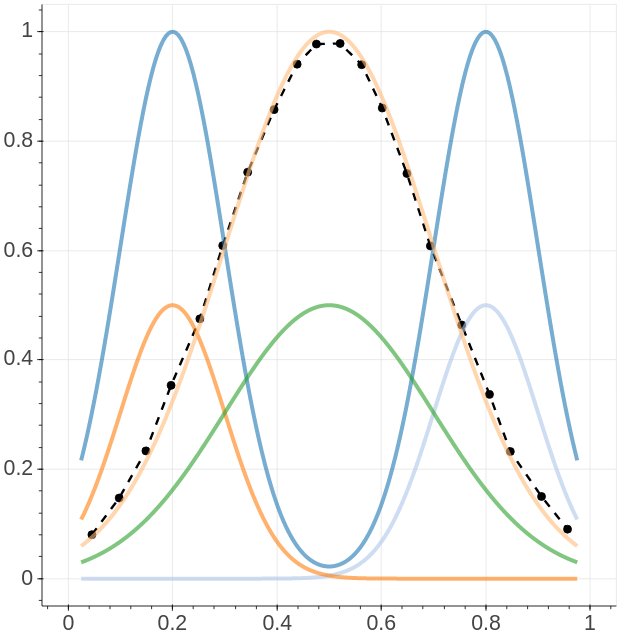
\includegraphics[height=4.5cm]{img/STEP1/gn1.png} \label{step1_4}}
    \subfigure{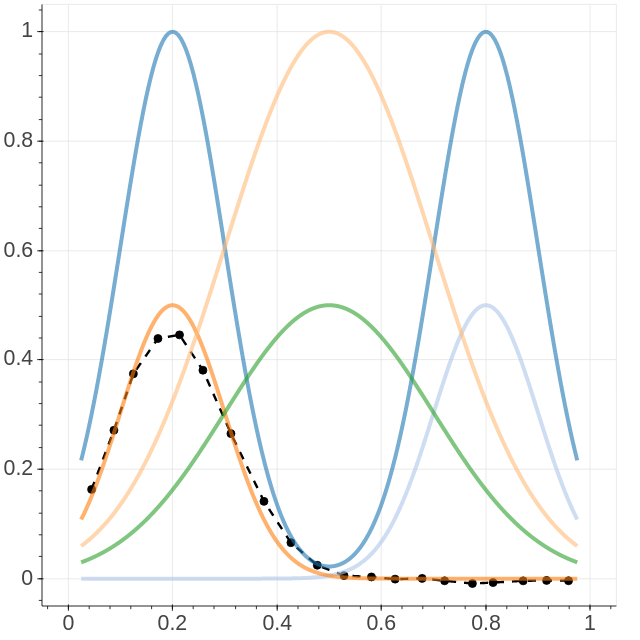
\includegraphics[height=4.5cm]{img/STEP1/gn2.png} \label{step1_5}}
    \subfigure{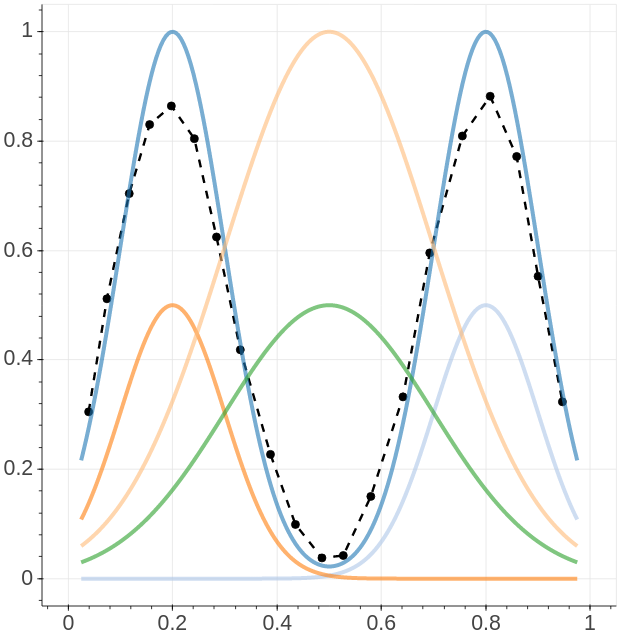
\includegraphics[height=4.5cm]{img/STEP1/gn3.png} \label{step1_6}}
    \caption{ STEP1 ls/gn }
    \label{fig:step_1}
\end{figure}


\section{Latent space regularization}

\section{Constraining regularizer with semi-supervised training}
